\documentclass[../main.tex]{subfiles}

\begin{document}

\chapter{Об’єктно-орієнтоване проектування ІС}

Якщо аналіз об’єкта проектування – це розробка відповідної логічної моделі, яка описує усі можливі та прийнятні варіанти розв’язання задач, які вказують, що повинна робити система, то проектування – це вироблення рішення відповідно до моделі аналізу, яке оптимізує набір критеріїв проектування, які  показують, як ця поведінка (робота) системи може бути реалізована \cite{diploma_guidelines}.
Оскільки, у даній роботі застосовується об’єктно-орієнтована технологія проектування, то проектна частина повинна складатися із таких етапів:

\begin{enumerate}
	\item Архітектурне проектування – описує логічну структуру інформаційної системи правильного харчування (програмні класи, підсистеми,  пакети) та їх зв’язки.
	\item Детальне проектування – описує структури даних та алгоритми всередині окремих класів. 
\end{enumerate}

\section{Архітектурне проектування}
Формування архітектури – перший і основний крок у розв’язанні завдання проектування, що закладає фундамент уявлення програмної системи, здатної виконувати весь спектр детальних вимог. \cite{diploma_guidelines2}

Створення архітектури – це проектування на найвищому рівні (логічна архітектура). Логічна архітектура описує систему в термінах її принципової організації у вигляді пакетів, програмних класів і підсистем. Вона називається логічною, оскільки не визначає способи розгортання цих елементів у різних операційних системах або на фізичних комп’ютерах в мережі (це відноситься до архітектури розгортання) \cite{diploma_guidelines}.

Одним з найважливіших етапів архітектурного проектування є побудова діаграми пакетів. 

Діаграма пакетів є діаграмою, яка містить пакети класів і залежності між ними. Вона описує архітектурну основу системи і допомагає в управлінні масштабами і складністю системи.

Діаграма пакетів для інформаційної системи зображена на рис. \ref{diagram:3.1}
\vspace{\baselineskip}

%TODO: change diagram after refactoring

\begin{figure}[H]
	\centering
	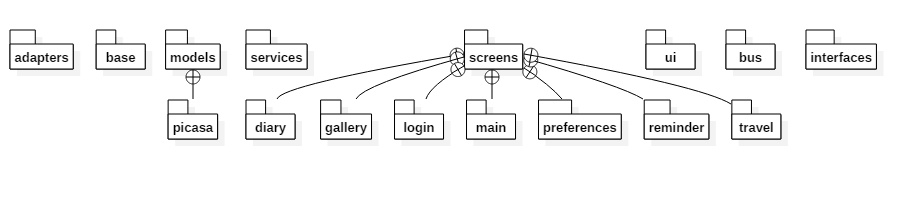
\includegraphics[width=1\textwidth]{diagram_packages}
	\caption{Діаграма пакетів інформаційної системи}
	\label{diagram:3.1}
\end{figure}

\section{Детальне проектування}

\begin{figure}[H]
	\centering
	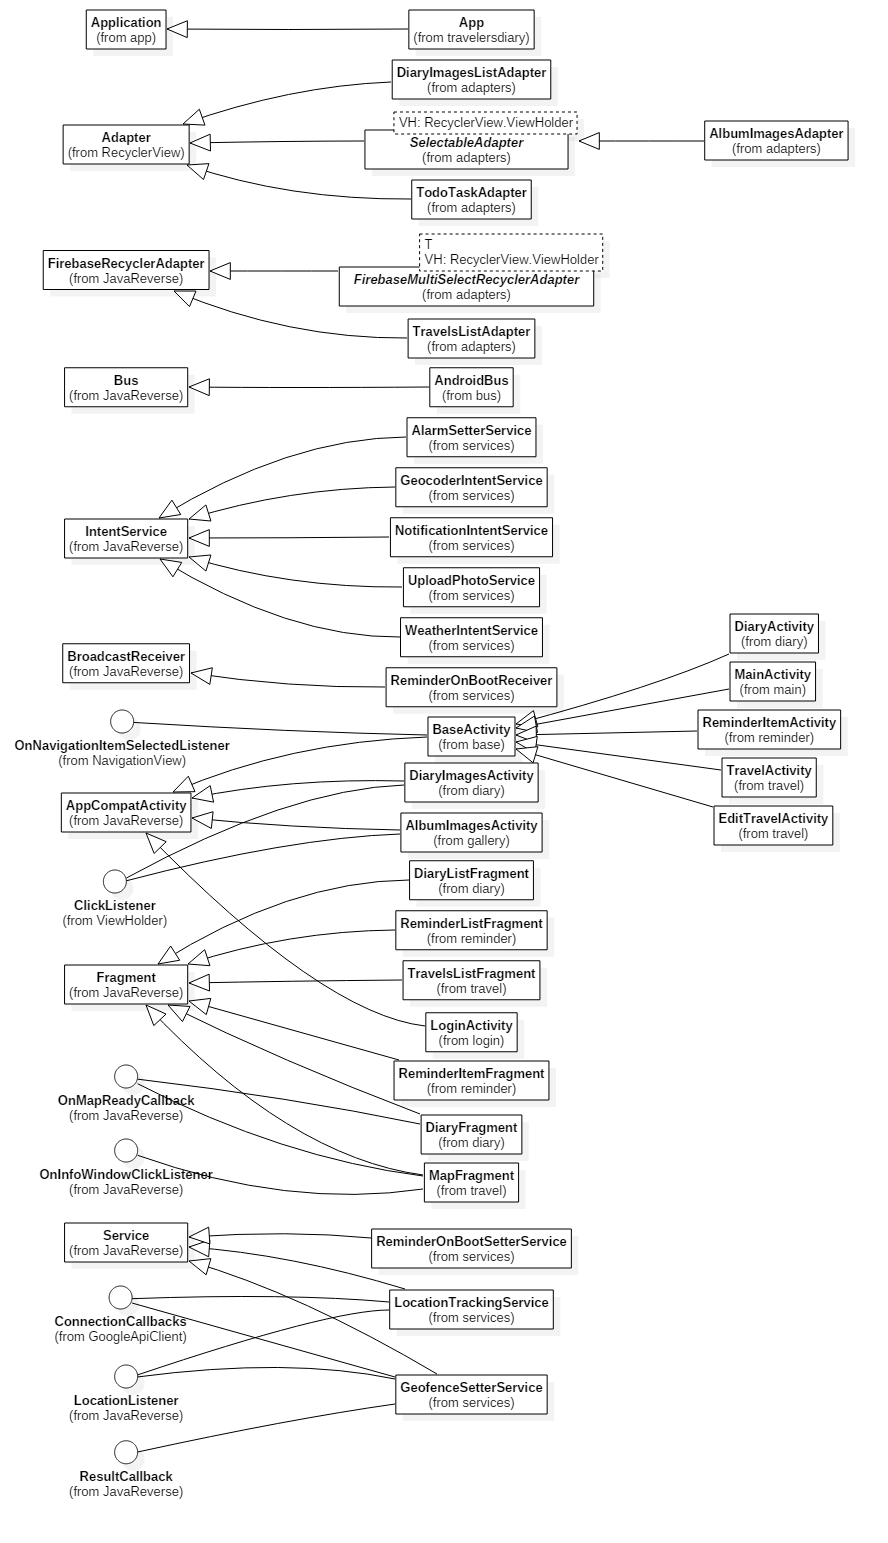
\includegraphics[height=0.8\textheight]{diagram_hierarchy}
	\caption{Діаграма компонентів Android додатку}
\end{figure}

\begin{figure}[H]
	\centering
	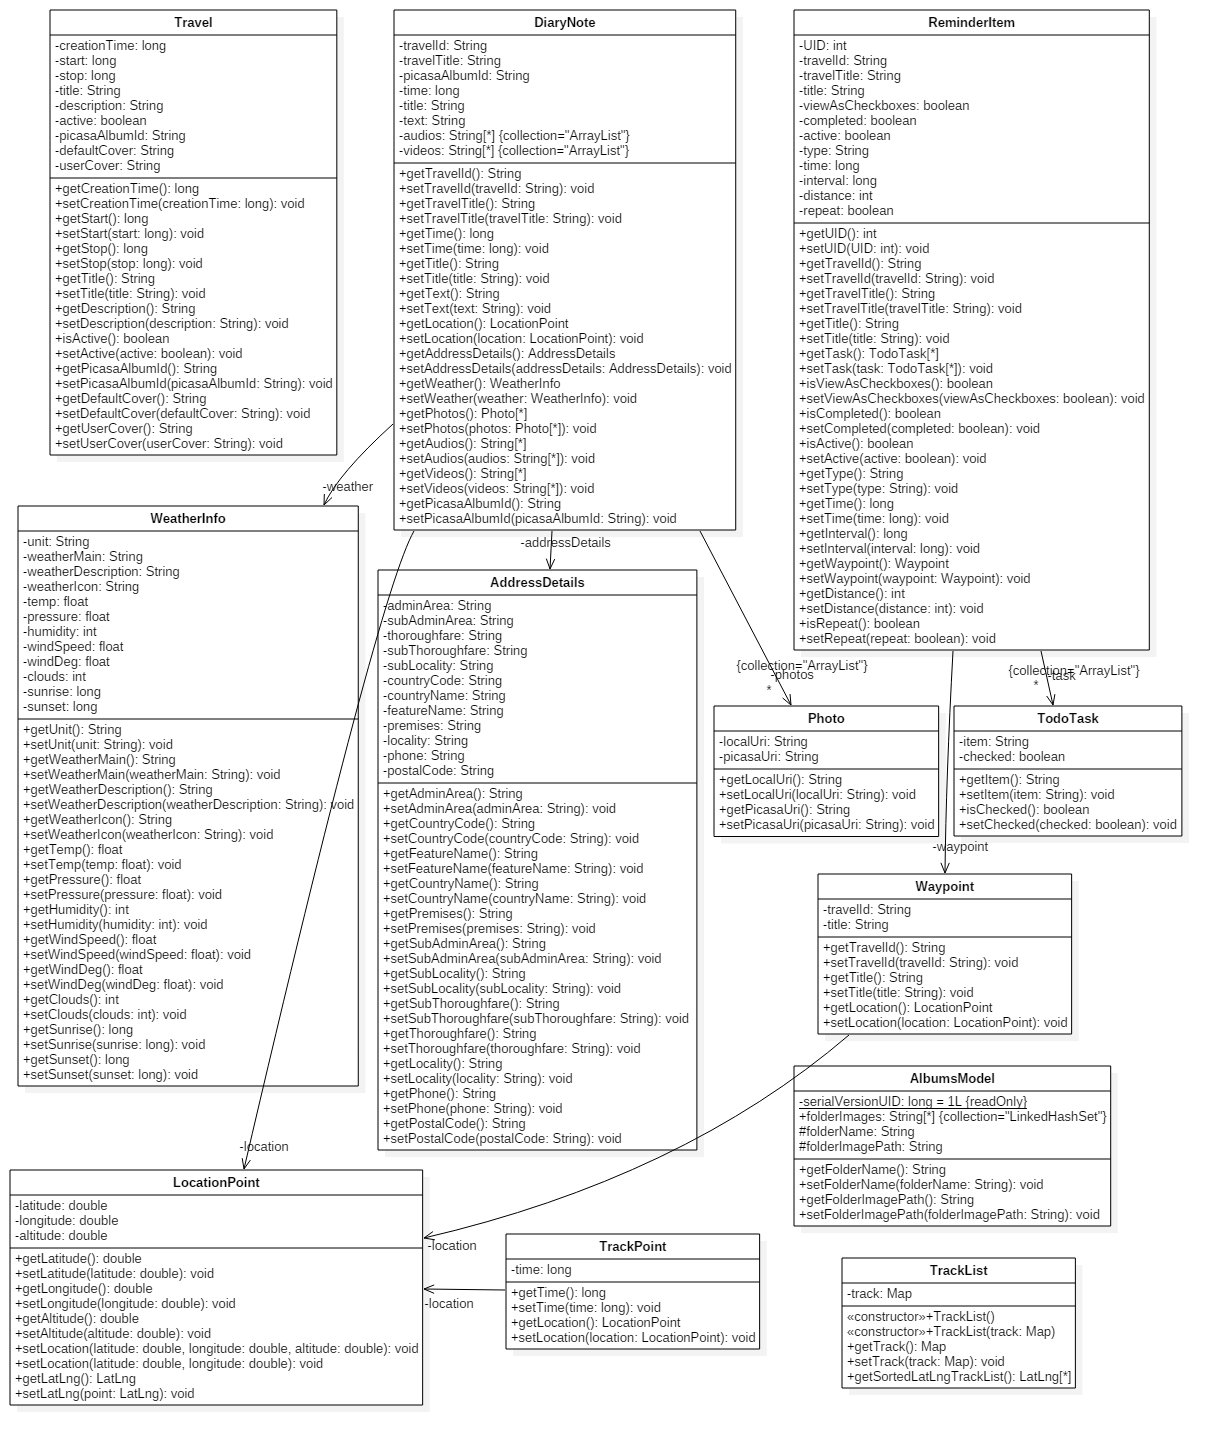
\includegraphics[height=0.8\textheight]{diagram_models}
	\caption{Діаграма моделей}
\end{figure}

\end{document}